\usetikzlibrary{arrows.meta}
\usetikzlibrary{calc}
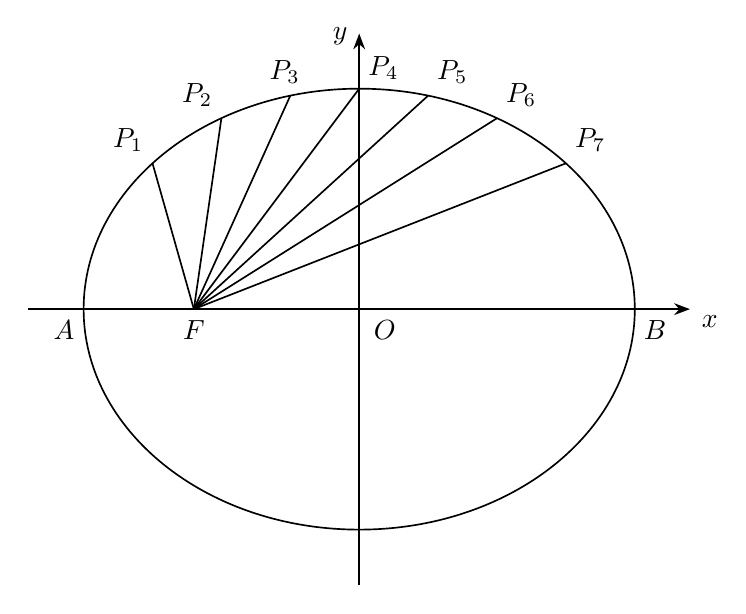
\begin{tikzpicture}[x=0.7cm,y=0.7cm,line width=.6pt,font=\normalsize,every node/.style={inner sep=0pt},>=Stealth]
\coordinate (A) at (-5,0);
\coordinate (B) at (5,0);
\coordinate (O) at (0,0);
\coordinate (F) at (-3,0);
\coordinate (P1) at (-3.75,2.645751311065);
\coordinate (P2) at (-2.5,3.464101615138);
\coordinate (P3) at (-1.25,3.872983346207);
\coordinate (P4) at (0,4.0);
\coordinate (P5) at (1.25,3.872983346207);
\coordinate (P6) at (2.5,3.464101615138);
\coordinate (P7) at (3.75,2.645751311065);
\coordinate (Xtip) at (6,0);
\coordinate (Ytip) at (0,5);
\draw[solid] (0,0) ellipse [x radius=5, y radius=4];
\draw (F) -- (P1);
\draw (F) -- (P2);
\draw (F) -- (P3);
\draw (F) -- (P4);
\draw (F) -- (P5);
\draw (F) -- (P6);
\draw (F) -- (P7);
\draw[->] (-6,0) -- (Xtip);
\draw[->] (0,-5) -- (Ytip);
\node[anchor=north east,inner sep=0pt] at ([xshift=-3pt,yshift=-4pt]A) {$A$};
\node[anchor=north west,inner sep=0pt] at ([xshift=3pt,yshift=-4pt]B) {$B$};
\node[anchor=north,inner sep=0pt] at ([yshift=-4pt]F) {$F$};
\node[anchor=north west,inner sep=0pt] at ([xshift=5pt,yshift=-4pt]O) {$O$};
\node[anchor=south east,inner sep=0pt] at ([xshift=-3pt,yshift=4pt]P1) {$P_{1}$};
\node[anchor=south east,inner sep=0pt] at ([xshift=-3pt,yshift=4pt]P2) {$P_{2}$};
\node[anchor=south,inner sep=0pt] at ([xshift=-2pt,yshift=4pt]P3) {$P_{3}$};
\node[anchor=south west,inner sep=0pt] at ([xshift=3pt,yshift=3pt]P4) {$P_{4}$};
\node[anchor=south west,inner sep=0pt] at ([xshift=3pt,yshift=4pt]P5) {$P_{5}$};
\node[anchor=south west,inner sep=0pt] at ([xshift=3pt,yshift=4pt]P6) {$P_{6}$};
\node[anchor=south west,inner sep=0pt] at ([xshift=3pt,yshift=4pt]P7) {$P_{7}$};
\node[anchor=north west,inner sep=0pt] at ([xshift=4pt,yshift=-2pt]Xtip) {$x$};
\node[anchor=east,inner sep=0pt] at ([xshift=-4pt,yshift=-1pt]Ytip) {$y$};
\end{tikzpicture}
